\documentclass[aspectratio=1610]{beamer}

\usetheme[titleformat=allsmallcaps]{metropolis}

% KAIST mtheme style.
\usepackage{kaist}

\usepackage{preamble}

\title{Cartesian Dualism}
\subtitle{Mind Distinct from Body}
\date{\today}
\author{Robin Eklind}
\titlegraphic{
\includegraphics[width=0.20\textwidth]{kaistgraphics/KAIST_logo_tran.png}}

\begin{document}

% --- [ Title ] ----------------------------------------------------------------

\maketitle

% --- [ Disposition ] ----------------------------------------------------------

\begin{frame}{Disposition}
	\begin{enumerate}
		%\item René Descartes on Doubt
		%\item Mental Causation
		\item Substance Dualism
		\item Arguments and Counter-arguments
			% I can doubt the existance of my body, but not that of my mind. Therefore they are not the same.
			% the pairing problem
		\item Final Thoughts
	\end{enumerate}
\end{frame}

% === [ Substance Dualism ] ====================================================

\section{Substance Dualism}

% --- [ I think, therefore I am ] ----------------------------------------------

\begin{frame}{I think, therefore I am}
	\begin{quote}
		\textit{``I can doubt the existance of my body, but because I think, I cannot doubt the existance of my mind.''}
		- René Descartes {\tiny (paraphrased)}
	\end{quote}

	\pause
	\vspace{2em}

	\textbf{``cogito'' Argument}: Since we can doubt the existance of one, but not the other, mind and body cannot be identical.

	\pause
	\vspace{2em}

	\emph{Therefore}, we are made of two fundamentally \textbf{distinct} substances:
	\begin{itemize}
		\item \alert{Res extensa}: material thing (extended in space)
		\item \alert{Res cogitans}: thinking thing
	\end{itemize}

\end{frame}

% --- [ What is a Substance? ] -------------------------------------------------

\begin{frame}{What is a Substance?}
	By definition, a \alert{substance} can exist \emph{independently} without any other substance.

	\begin{itemize}
		\pause
		\item Matter can exist without a mind (e.g. a rock).
		\pause
		\item A mind can \textit{in principle} exist without a body.
	\end{itemize}
\end{frame}

% --- [ Where is the Mind? ] ---------------------------------------------------

\begin{frame}{Where is the Mind?}
	Nowadays considered a historical anecdote, René Descartes believed the \alert{pineal gland} to the \textit{principal seat of the soul}, through which the mind interacted with the body.

	\begin{figure}
		\centering
		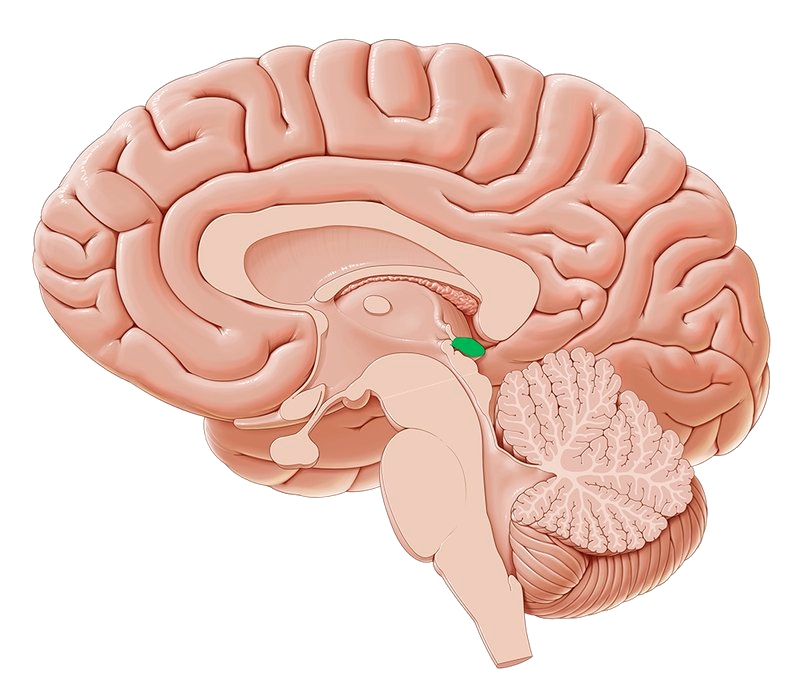
\includegraphics[height=0.55\paperheight]{inc/pineal_gland.png}
		\caption{The pineal gland of the brain.}
	\end{figure}
\end{frame}

% === [ Arguments and Counter-arguments ] ======================================

\section{Arguments and Counter-arguments}

% --- [ Frame Three ] ----------------------------------------------------------

\begin{frame}{Frame Three}
	foo
\end{frame}

% --- [ Frame Four ] -----------------------------------------------------------

\begin{frame}{Frame Four}
	foo
\end{frame}

% --- [ Frame Five ] -----------------------------------------------------------

\begin{frame}{Frame Five}
	foo
\end{frame}

% === [ Questions ] ============================================================

\begin{frame}[standout]
	Questions?
\end{frame}

\end{document}
